\section{Results and Tests}
\subsection{uClinux}
After building and flashing \emph{uClinux} on the chip, we verified that we had a working Linux distribution by connecting to its shell with \emph{miniterm.py} and running Linux commands like \emph{ls} and \emph{cat}. In addition to this, we saw Tux on the screen, indicating that \emph{uClinux} was properly installed.

\subsection{Gamepad driver}
\begin{figure}[h]
	\centering
	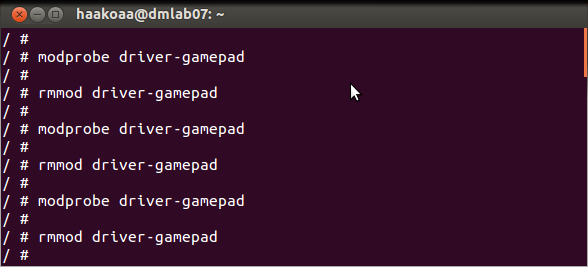
\includegraphics[width=12cm]{img/modprobe.png}
	\caption{Adding and removing the module several times}
	\label{fig:modprobe}
\end{figure}
Testing that the gamepad driver delivers the correct data to the user space is left to our game. If the game functions as expected, we can therefore conclude that the gamepad driver reads and delivers the correct data. Please read on (section \ref{subsection:pong-testing}) to verify the correctness of this.\\
\\
In addition to delivering the correct data on time, it is really important that the driver cleans up properly by deallocating and freeing various data structures used for it's operation. Failing to do so, might cause memory leaks in kernel space; a situation where memory does not get freed before system reboot. Besides from being very accurate (making sure each allocation call had a corresponding deallocation call) in writing the drivers probe and close functions, we tested that we were able to load and uload our kernel module multiple times. We did a test by calling \emph{modprobe driver-gamepad} and \emph{rmmod driver-gamepad} consecutively three times, checking that neither of the calls yielded any error messages. As we can see in figure \ref{fig:modprobe}, the test was a success.

\subsection{Pong}
\label{subsection:pong-testing}
It is always important to have a system that behaves as expected, so our game 
As usual, we 
\begin{itemize}
	\item At spillet ikke lagger
	\item At ballen spretter fint av kantene og spillerne
	\item At spillet resetter seg når man er ferdig
\end{itemize}

\subsection{Energy efficiency and performance}

\subsubsection{Performance and energy efficiency with different frame update modes}

\subsubsection{Tickless idle}
